\documentclass{article}
\usepackage{ctex}
\usepackage{graphicx}
\usepackage{amsmath}
\usepackage{indentfirst}
\usepackage{titlesec}
\usepackage{setspace}
\usepackage{subfigure}
\usepackage{caption}
\usepackage{float}
\usepackage{booktabs}
\usepackage{geometry}
\usepackage{multirow}
\geometry{left=1.2cm,right=1.2cm,top=2cm,bottom=2cm}
\title{\songti \zihao{2}\bfseries HW4Jacobi方法}
\titleformat*{\section}{\songti\zihao{4}\bfseries}
\titleformat*{\subsection}{\songti\zihao{5}\bfseries}
\renewcommand\thesection{\arabic{section}}
\author{王启骅 PB20020580}
\begin{document}
	\maketitle
	
	\section{实验结果与分析}
	
	\subsection{SVD分解}
	生成的初始矩阵如图1
		\begin{figure}[!h]
		
		\centering
		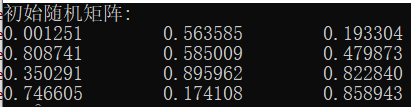
\includegraphics[scale=1]{A}
		\captionsetup{font={small},labelfont=bf}
		\caption{\heiti\zihao{-5}初始矩阵A}
		
	\end{figure}


	计算得到$ AA^T $并使用Jacobi方法得到对角特征值矩阵结果为图2
		\begin{figure}[!h]
		
		\centering
		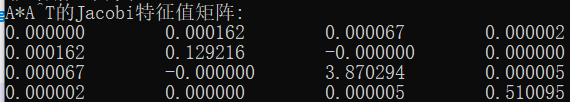
\includegraphics[scale=1]{EV}
		\captionsetup{font={small},labelfont=bf}
		\caption{\heiti\zihao{-5}$ AA^T $的Jacobi方法结果特征值对角矩阵}
		
	\end{figure}


得到迭代过程中每次的非对角元平方和如图3,可见非对角元平方和确实每次都呈迅速下降趋势。
	\begin{figure}[!h]
	
	\centering
	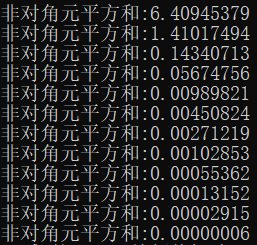
\includegraphics[scale=1]{square_sum}
	\captionsetup{font={small},labelfont=bf}
	\caption{\heiti\zihao{-5}非对角元平方和}
	
\end{figure}


最后输出变换矩阵Q即为所需的U,再计算SIGMA与V得到结果如图4
	\begin{figure}[!h]
	
	\centering
	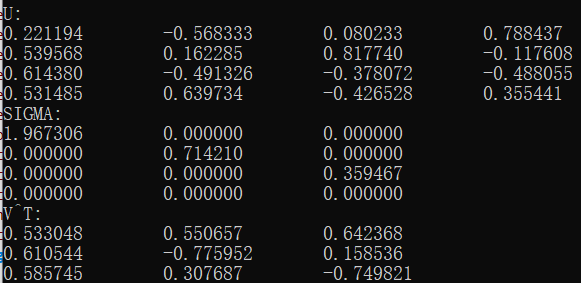
\includegraphics[scale=1]{U_SIGMA_V}
	\captionsetup{font={small},labelfont=bf}
	\caption{\heiti\zihao{-5} $U\ \Sigma \ V$矩阵}
	
\end{figure}


接下来按照图2所求的特征值矩阵对角元顺序一次求$ det(AA^T-\lambda_iI) $得到结果如图5,如图可见该行列式绝对值计算结果均小于$ 10^{-7} $次方,趋于0,可见所求结果确实为正确的矩阵特征值。
	\begin{figure}[!h]
	
	\centering
	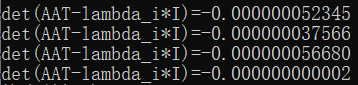
\includegraphics[scale=1]{det}
	\captionsetup{font={small},labelfont=bf}
	\caption{\heiti\zihao{-5}$ det(AA^T-\lambda_iI) $}
	
\end{figure}

	\subsection{PCA分析}
	所求得到$ \frac{1}{m}XX^T $协方差矩阵为图6
		\begin{figure}[!h]
		
		\centering
		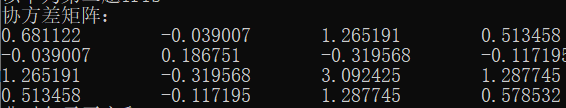
\includegraphics[scale=1]{cov}
		\captionsetup{font={small},labelfont=bf}
		\caption{\heiti\zihao{-5}$ \frac{1}{m}XX^T $}
		
	\end{figure}


计算其特征值、特征向量矩阵为图6,7	
\begin{figure}[!h]
	
	\centering
	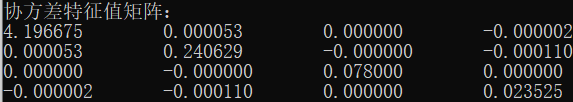
\includegraphics[scale=1]{cov_EV}
	\captionsetup{font={small},labelfont=bf}
	\caption{\heiti\zihao{-5}$ \frac{1}{m}XX^T $的特征值矩阵}
	
\end{figure}
\begin{figure}[!h]
	
	\centering
	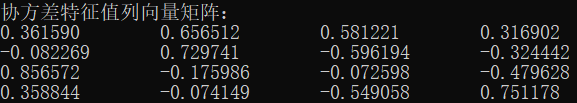
\includegraphics[scale=1]{vec}
	\captionsetup{font={small},labelfont=bf}
	\caption{\heiti\zihao{-5}$ \frac{1}{m}XX^T $的特征向量矩阵}
	
\end{figure}


将生成的投影坐标输出到coordinate.txt,读入到python文件Cov pic.py画图得到可视化结果如图8,其中前50个点对应蓝色,50-100对应红色,100-150对应绿色
	\begin{figure}[!h]
	
	\centering
	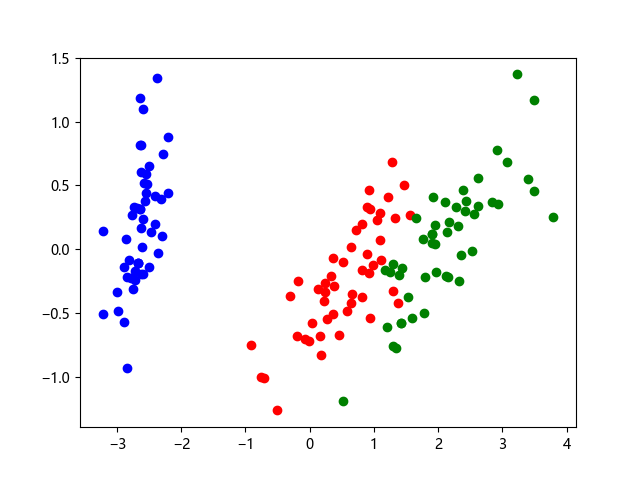
\includegraphics[scale=1]{iris}
	\captionsetup{font={small},labelfont=bf}
	\caption{\heiti\zihao{-5}IRIS可视化结果}
	
\end{figure}


可见对于第0组数据点,其特征向量投影再靠近x=-3,y=$ -1\sim 1.5 $的位置附近,说明第0组数据在$ \hat{e_1} $方向的投影相近,都在-3左右,而在$ \hat{e_2} $方向投影差异较大;对于第1组数据,可见其主要分布在近似于y=x的靠近原点的直线上,说明其数据大多分布在朝向$ \hat{e_1},\hat{e_2} $方向之间的某一夹角的方向正负附近;对于第2组数据,其主要分布在4>x>0,1.5>y>-1.5的区域,也主要沿y=x的方向分布,说明该组数据在$ \hat{e_1} $方向投影均为正值,说明数据相对$ \hat{e_1} $的方向不改变,而相对$ \hat{e_2} $则总体上随对$ \hat{e_1} $的投影增大而增大的趋势。由此可见三组数据明显属于不同种类的花,有不同特性。
\end{document}